\documentclass[../../main]{subfiles}


\begin{document}
This semester projects main theme is centered around the control of a dynamic system. using control theory The system itself is a pan tilt system, shown below in figure \ref{figure_pantil}. The usecase, decided by the group for the project, is mounting a stage lamp onto the system for use in theatre or similar setting. The angle of the light is controlled through a interface built around input from a ???? connected to a computer. The usecase is only theoretical and use to have a goal to work towards and requrements for the control theory aspects, meaning that a lamp will never be mounted on the system. The pan tilt system is provided assembled and requres in this project no further physical alterations. This means the project will only be describing the software and control theory decisions required to achieve a functioning pan tilt system for a stage lamp. The software will be divivded into three parts; one part written for a  FPGA xxx, one part is for a tiva C series xx and the last part is for a genreic laptop/computer. The computer part contains the UI and interface for the application used to control the system and provide any useful feedback, positiion or velocity of the systerm, for the user. The Tiva will be progreammed in C and function as the heart of the system with the control theory implemented here and an SPI connecting  itself and the FPGA. The Tiva's porpuse will esssentially be to control the system through the FPGA The FPGA will be responsible for obtaining the position from the systems two encoders and controlling the systems motors with a PWM signal recieved from the Tiva. 

\subsection*{Bud fra Lasse}

This semester project revolves around the control of a dynamic system, more specific a pan-tilt  system shown in figure \ref{fig:system}.

\begin{figure}[H]
\centering
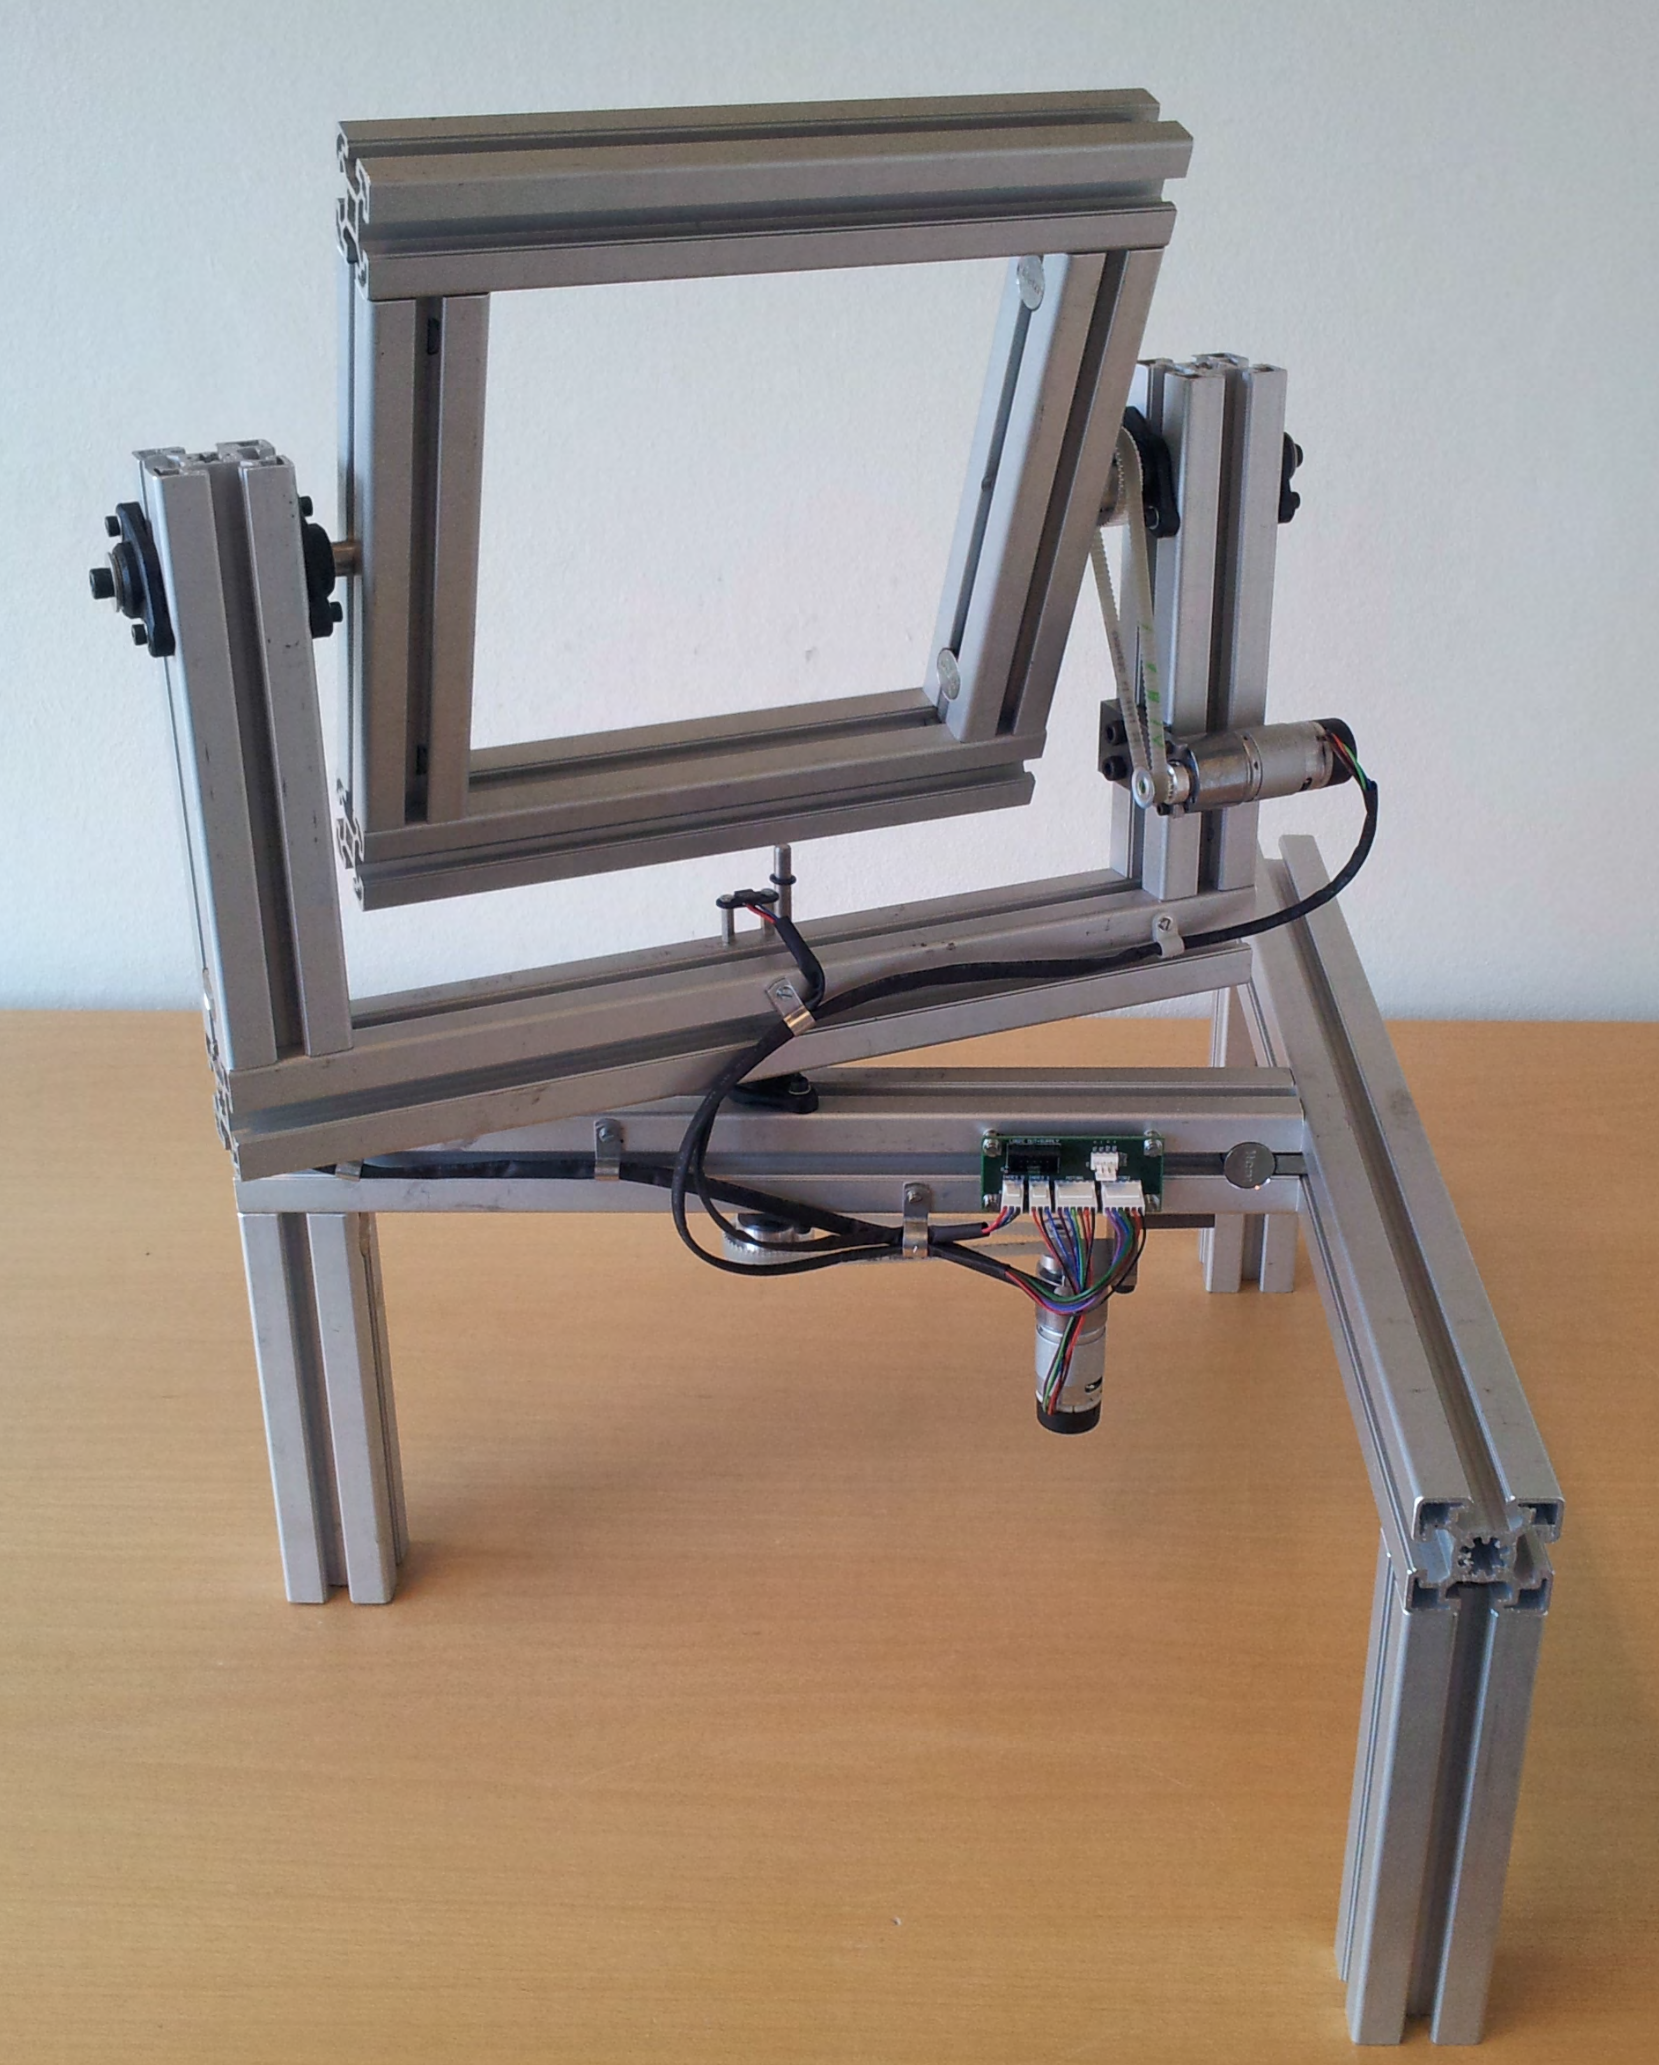
\includegraphics[width=0.5\textwidth]{\main/afsnit/introduction/images/pantilt.png}
\caption{Pan-Tilt system}
\label{fig:system}
\end{figure}

The use case, defined by the group for the project, is mounting a stage lamp onto the system for use in theater or similar setting.
The angle of the light is controlled on both the pan and tilt axis through an interface with the Tiva microcontroller, either using the UART connection or the hardware input devices directly attached, these devices can be seen in figure \ref{fig:empboard}  

\begin{figure}[H]
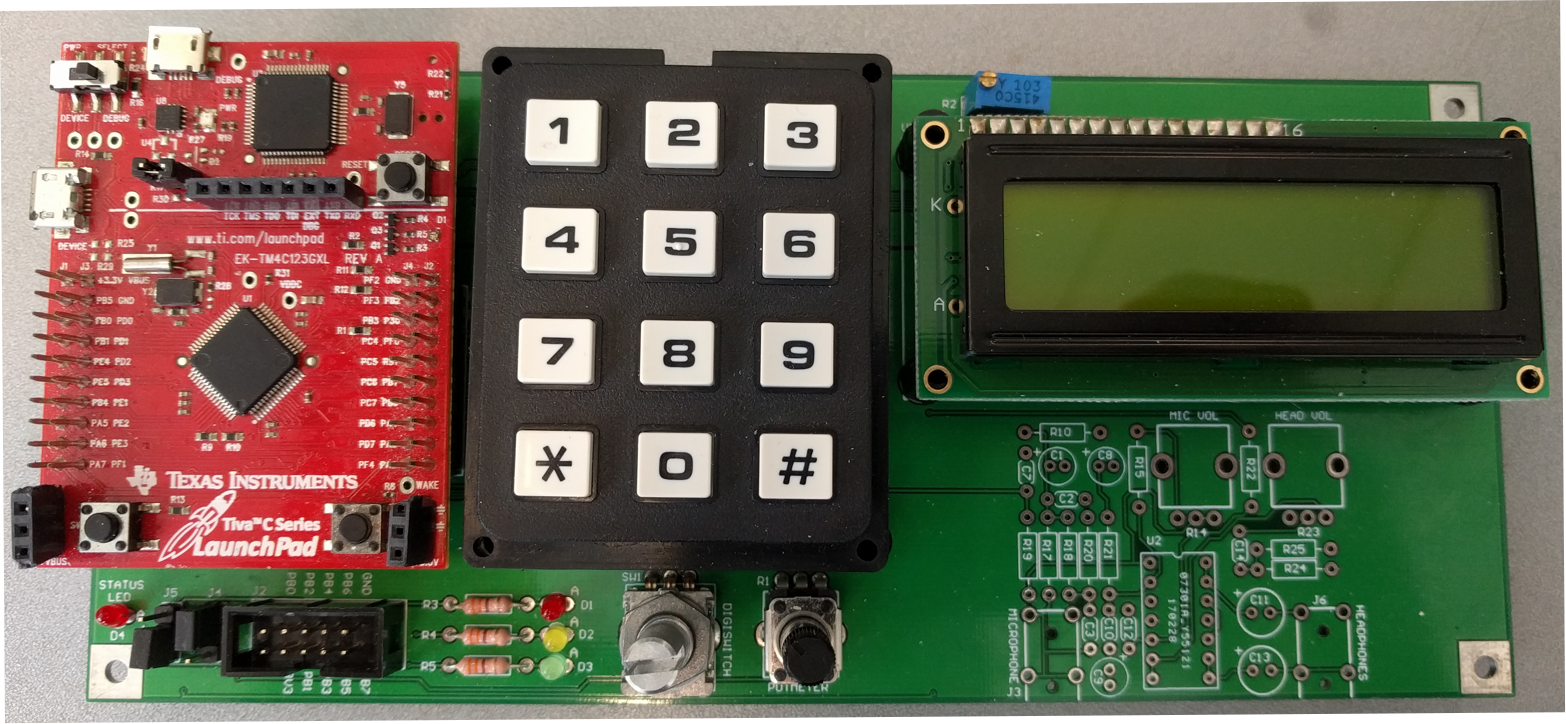
\includegraphics[width=\textwidth]{\main/afsnit/introduction/images/empboard.png}
\caption{EMP board provided to the project}
\label{fig:empboard}
\end{figure}

The use case is exclusively theoretical and aims to set the requirements for the system.
The pan tilt system is provided assembled and requires no further physical alterations. The scope of the project is therefore limited to software and control engineering decisions required to achieve a conforming, to set requirements, pan-tilt system for a stage lamp.

The project will be run on a Tiva ??? microcontroller and a Artix-7 FPGA. Software must be designed and written to allow these devices, in tandem to control the pan-tilt system to move in a coordinated fashion. 
The Tiva microcontroller will have software written in C while the FPGA behavior is defined using VHDL. The Tiva will control most of the logic of the system while the FPGA acts mainly as a hardware controller and data acquisitions device. 

\end{document}
